% Created by tikzDevice version 0.12.3 on 2020-01-17 15:18:24
% !TEX encoding = UTF-8 Unicode
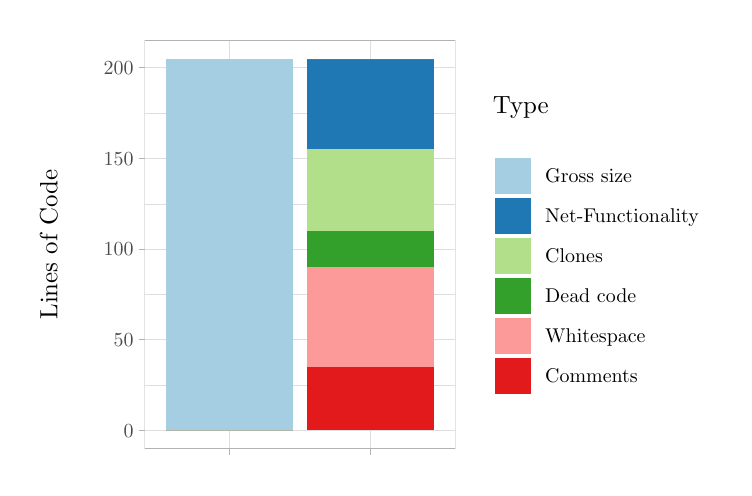
\begin{tikzpicture}[x=1pt,y=1pt]
\definecolor{fillColor}{RGB}{255,255,255}
\path[use as bounding box,fill=fillColor,fill opacity=0.00] (0,0) rectangle (251.50,158.99);
\begin{scope}
\path[clip] (  0.00,  0.00) rectangle (251.50,158.99);
\definecolor{drawColor}{RGB}{255,255,255}
\definecolor{fillColor}{RGB}{255,255,255}

\path[draw=drawColor,line width= 0.5pt,line join=round,line cap=round,fill=fillColor] (  0.00,  0.00) rectangle (251.50,158.99);
\end{scope}
\begin{scope}
\path[clip] ( 42.30,  6.75) rectangle (154.56,154.49);
\definecolor{fillColor}{RGB}{255,255,255}

\path[fill=fillColor] ( 42.30,  6.75) rectangle (154.56,154.49);
\definecolor{drawColor}{gray}{0.87}

\path[draw=drawColor,line width= 0.1pt,line join=round] ( 42.30, 29.85) --
	(154.56, 29.85);

\path[draw=drawColor,line width= 0.1pt,line join=round] ( 42.30, 62.60) --
	(154.56, 62.60);

\path[draw=drawColor,line width= 0.1pt,line join=round] ( 42.30, 95.36) --
	(154.56, 95.36);

\path[draw=drawColor,line width= 0.1pt,line join=round] ( 42.30,128.12) --
	(154.56,128.12);

\path[draw=drawColor,line width= 0.2pt,line join=round] ( 42.30, 13.47) --
	(154.56, 13.47);

\path[draw=drawColor,line width= 0.2pt,line join=round] ( 42.30, 46.22) --
	(154.56, 46.22);

\path[draw=drawColor,line width= 0.2pt,line join=round] ( 42.30, 78.98) --
	(154.56, 78.98);

\path[draw=drawColor,line width= 0.2pt,line join=round] ( 42.30,111.74) --
	(154.56,111.74);

\path[draw=drawColor,line width= 0.2pt,line join=round] ( 42.30,144.50) --
	(154.56,144.50);

\path[draw=drawColor,line width= 0.2pt,line join=round] ( 72.91,  6.75) --
	( 72.91,154.49);

\path[draw=drawColor,line width= 0.2pt,line join=round] (123.94,  6.75) --
	(123.94,154.49);
\definecolor{fillColor}{RGB}{227,26,28}

\path[fill=fillColor] ( 49.95, 13.47) rectangle ( 95.88, 13.47);
\definecolor{fillColor}{RGB}{251,154,153}

\path[fill=fillColor] ( 49.95, 13.47) rectangle ( 95.88, 13.47);
\definecolor{fillColor}{RGB}{51,160,44}

\path[fill=fillColor] ( 49.95, 13.47) rectangle ( 95.88, 13.47);
\definecolor{fillColor}{RGB}{178,223,138}

\path[fill=fillColor] ( 49.95, 13.47) rectangle ( 95.88, 13.47);
\definecolor{fillColor}{RGB}{31,120,180}

\path[fill=fillColor] ( 49.95, 13.47) rectangle ( 95.88, 13.47);
\definecolor{fillColor}{RGB}{166,206,227}

\path[fill=fillColor] ( 49.95, 13.47) rectangle ( 95.88,147.78);
\definecolor{fillColor}{RGB}{227,26,28}

\path[fill=fillColor] (100.98, 13.47) rectangle (146.90, 36.40);
\definecolor{fillColor}{RGB}{251,154,153}

\path[fill=fillColor] (100.98, 36.40) rectangle (146.90, 72.43);
\definecolor{fillColor}{RGB}{51,160,44}

\path[fill=fillColor] (100.98, 72.43) rectangle (146.90, 85.54);
\definecolor{fillColor}{RGB}{178,223,138}

\path[fill=fillColor] (100.98, 85.54) rectangle (146.90,115.02);
\definecolor{fillColor}{RGB}{31,120,180}

\path[fill=fillColor] (100.98,115.02) rectangle (146.90,147.78);
\definecolor{fillColor}{RGB}{166,206,227}

\path[fill=fillColor] (100.98,147.78) rectangle (146.90,147.78);
\definecolor{drawColor}{gray}{0.70}

\path[draw=drawColor,line width= 0.5pt,line join=round,line cap=round] ( 42.30,  6.75) rectangle (154.56,154.49);
\end{scope}
\begin{scope}
\path[clip] (  0.00,  0.00) rectangle (251.50,158.99);
\definecolor{drawColor}{gray}{0.30}

\node[text=drawColor,anchor=base east,inner sep=0pt, outer sep=0pt, scale=  0.72] at ( 38.25, 10.99) {0};

\node[text=drawColor,anchor=base east,inner sep=0pt, outer sep=0pt, scale=  0.72] at ( 38.25, 43.75) {50};

\node[text=drawColor,anchor=base east,inner sep=0pt, outer sep=0pt, scale=  0.72] at ( 38.25, 76.50) {100};

\node[text=drawColor,anchor=base east,inner sep=0pt, outer sep=0pt, scale=  0.72] at ( 38.25,109.26) {150};

\node[text=drawColor,anchor=base east,inner sep=0pt, outer sep=0pt, scale=  0.72] at ( 38.25,142.02) {200};
\end{scope}
\begin{scope}
\path[clip] (  0.00,  0.00) rectangle (251.50,158.99);
\definecolor{drawColor}{gray}{0.70}

\path[draw=drawColor,line width= 0.2pt,line join=round] ( 40.05, 13.47) --
	( 42.30, 13.47);

\path[draw=drawColor,line width= 0.2pt,line join=round] ( 40.05, 46.22) --
	( 42.30, 46.22);

\path[draw=drawColor,line width= 0.2pt,line join=round] ( 40.05, 78.98) --
	( 42.30, 78.98);

\path[draw=drawColor,line width= 0.2pt,line join=round] ( 40.05,111.74) --
	( 42.30,111.74);

\path[draw=drawColor,line width= 0.2pt,line join=round] ( 40.05,144.50) --
	( 42.30,144.50);
\end{scope}
\begin{scope}
\path[clip] (  0.00,  0.00) rectangle (251.50,158.99);
\definecolor{drawColor}{gray}{0.70}

\path[draw=drawColor,line width= 0.2pt,line join=round] ( 72.91,  4.50) --
	( 72.91,  6.75);

\path[draw=drawColor,line width= 0.2pt,line join=round] (123.94,  4.50) --
	(123.94,  6.75);
\end{scope}
\begin{scope}
\path[clip] (  0.00,  0.00) rectangle (251.50,158.99);
\definecolor{drawColor}{RGB}{0,0,0}

\node[text=drawColor,rotate= 90.00,anchor=base,inner sep=0pt, outer sep=0pt, scale=  0.90] at ( 10.70, 80.62) {Lines of Code};
\end{scope}
\begin{scope}
\path[clip] (  0.00,  0.00) rectangle (251.50,158.99);
\definecolor{fillColor}{RGB}{255,255,255}

\path[fill=fillColor] (163.56, 21.54) rectangle (247.00,139.71);
\end{scope}
\begin{scope}
\path[clip] (  0.00,  0.00) rectangle (251.50,158.99);
\definecolor{drawColor}{RGB}{0,0,0}

\node[text=drawColor,anchor=base west,inner sep=0pt, outer sep=0pt, scale=  0.90] at (168.06,128.13) {Type};
\end{scope}
\begin{scope}
\path[clip] (  0.00,  0.00) rectangle (251.50,158.99);
\definecolor{fillColor}{RGB}{255,255,255}

\path[fill=fillColor] (168.06, 98.31) rectangle (182.51,112.76);
\end{scope}
\begin{scope}
\path[clip] (  0.00,  0.00) rectangle (251.50,158.99);
\definecolor{fillColor}{RGB}{166,206,227}

\path[fill=fillColor] (168.77, 99.02) rectangle (181.80,112.05);
\end{scope}
\begin{scope}
\path[clip] (  0.00,  0.00) rectangle (251.50,158.99);
\definecolor{fillColor}{RGB}{255,255,255}

\path[fill=fillColor] (168.06, 83.85) rectangle (182.51, 98.31);
\end{scope}
\begin{scope}
\path[clip] (  0.00,  0.00) rectangle (251.50,158.99);
\definecolor{fillColor}{RGB}{31,120,180}

\path[fill=fillColor] (168.77, 84.56) rectangle (181.80, 97.59);
\end{scope}
\begin{scope}
\path[clip] (  0.00,  0.00) rectangle (251.50,158.99);
\definecolor{fillColor}{RGB}{255,255,255}

\path[fill=fillColor] (168.06, 69.40) rectangle (182.51, 83.85);
\end{scope}
\begin{scope}
\path[clip] (  0.00,  0.00) rectangle (251.50,158.99);
\definecolor{fillColor}{RGB}{178,223,138}

\path[fill=fillColor] (168.77, 70.11) rectangle (181.80, 83.14);
\end{scope}
\begin{scope}
\path[clip] (  0.00,  0.00) rectangle (251.50,158.99);
\definecolor{fillColor}{RGB}{255,255,255}

\path[fill=fillColor] (168.06, 54.94) rectangle (182.51, 69.40);
\end{scope}
\begin{scope}
\path[clip] (  0.00,  0.00) rectangle (251.50,158.99);
\definecolor{fillColor}{RGB}{51,160,44}

\path[fill=fillColor] (168.77, 55.66) rectangle (181.80, 68.69);
\end{scope}
\begin{scope}
\path[clip] (  0.00,  0.00) rectangle (251.50,158.99);
\definecolor{fillColor}{RGB}{255,255,255}

\path[fill=fillColor] (168.06, 40.49) rectangle (182.51, 54.94);
\end{scope}
\begin{scope}
\path[clip] (  0.00,  0.00) rectangle (251.50,158.99);
\definecolor{fillColor}{RGB}{251,154,153}

\path[fill=fillColor] (168.77, 41.20) rectangle (181.80, 54.23);
\end{scope}
\begin{scope}
\path[clip] (  0.00,  0.00) rectangle (251.50,158.99);
\definecolor{fillColor}{RGB}{255,255,255}

\path[fill=fillColor] (168.06, 26.04) rectangle (182.51, 40.49);
\end{scope}
\begin{scope}
\path[clip] (  0.00,  0.00) rectangle (251.50,158.99);
\definecolor{fillColor}{RGB}{227,26,28}

\path[fill=fillColor] (168.77, 26.75) rectangle (181.80, 39.78);
\end{scope}
\begin{scope}
\path[clip] (  0.00,  0.00) rectangle (251.50,158.99);
\definecolor{drawColor}{RGB}{0,0,0}

\node[text=drawColor,anchor=base west,inner sep=0pt, outer sep=0pt, scale=  0.72] at (187.01,103.05) {Gross size};
\end{scope}
\begin{scope}
\path[clip] (  0.00,  0.00) rectangle (251.50,158.99);
\definecolor{drawColor}{RGB}{0,0,0}

\node[text=drawColor,anchor=base west,inner sep=0pt, outer sep=0pt, scale=  0.72] at (187.01, 88.60) {Net-Functionality};
\end{scope}
\begin{scope}
\path[clip] (  0.00,  0.00) rectangle (251.50,158.99);
\definecolor{drawColor}{RGB}{0,0,0}

\node[text=drawColor,anchor=base west,inner sep=0pt, outer sep=0pt, scale=  0.72] at (187.01, 74.15) {Clones};
\end{scope}
\begin{scope}
\path[clip] (  0.00,  0.00) rectangle (251.50,158.99);
\definecolor{drawColor}{RGB}{0,0,0}

\node[text=drawColor,anchor=base west,inner sep=0pt, outer sep=0pt, scale=  0.72] at (187.01, 59.69) {Dead code};
\end{scope}
\begin{scope}
\path[clip] (  0.00,  0.00) rectangle (251.50,158.99);
\definecolor{drawColor}{RGB}{0,0,0}

\node[text=drawColor,anchor=base west,inner sep=0pt, outer sep=0pt, scale=  0.72] at (187.01, 45.24) {Whitespace};
\end{scope}
\begin{scope}
\path[clip] (  0.00,  0.00) rectangle (251.50,158.99);
\definecolor{drawColor}{RGB}{0,0,0}

\node[text=drawColor,anchor=base west,inner sep=0pt, outer sep=0pt, scale=  0.72] at (187.01, 30.78) {Comments};
\end{scope}
\end{tikzpicture}
